\documentclass{beamer}


\setbeamertemplate{background canvas}[vertical shading][bottom=white,top=structure.fg!25]
% or whatever

\usetheme{Warsaw}
\setbeamertemplate{headline}{}
\setbeamertemplate{footline}{}
\setbeamersize{text margin left=0.5cm}
  
\usepackage[english]{babel}
% or whatever

\usepackage[utf8]{inputenc}
% or whatever

\usepackage{times}
\usepackage[T1]{fontenc}
% Or whatever. Note that the encoding and the font should match. If T1
% does not look nice, try deleting the line with the fontenc.

\usepackage{amsfonts}
\usepackage{amsmath,amsthm}
\usepackage{url}
\usepackage{pdfpages}


\title[Statistical test]
{Statistical test}
\author[Mirjam Pergar]
{\textbf{Student:}  Mirjam Pergar\\
\textbf{Proposer and mentor:} dr. asist. Gregor Šega
}
\institute[Fakuleta za matematiko in fiziko]

\date[April 20th 2017] % (optional)
{April 20th 2017}

\setbeamertemplate{footline}[frame number]
\begin{document}
\begin{frame}
\titlepage
\end{frame}

\begin{frame}{Description of the project}
\begin{enumerate}
\item Generate 
$$X_{1,1}, X_{1,2},X_{1,3}, \dots , X_{1,n}$$
$$\vdots$$
$$X_{r,1}, X_{r,2}, X_{r,3}, \dots, X_{r,n}$$
for a normally distributed random variable $X$ and some $r, n$.
\item Calculate sample variances $s^2_{1}, \dots, s^2_{r}$.
\item Test homoscedacity for significance level $\alpha$, for some $\alpha$.
\item Use the proposed statistical test: $$F =\frac{ \sum_{i=1}^{r} s^2_{(i)} \frac{2i-1}{r}}{\sum_{i=1}^{r} s^2_{(i)}}$$
\end{enumerate}
\end{frame}

\begin{frame}{Assumptions}
\begin{itemize}
\item $X \sim N(0,1)$
\item $n = \{2,3,4,\dots, 9,10,12,14,\dots, 18,20,25,30,40,60\}$
\item $r = \{2,3,4, \dots ,9,10,15,20\}$
\item $\alpha = \{1\%,5\%,10\%\}$
\end{itemize}
\pause
\begin{enumerate}[(a)]
\item How many times should we generate the random variables?
\item How long will this take?
\end{enumerate}

\end{frame}

\begin{frame}{Loops}
$n=2$, $r=2$\\
\only<1>{\centering \it 1e+3 loops}
\only<2>{\centering \it 1e+4 loops}
\only<3>{\centering \it 1e+5 loops}
\only<4>{\centering \it 1e+6 loops}
\only<5>{\centering \it 1e+7 loops}
\begin{figure}

\begin{overprint}
\onslide<1>\centerline{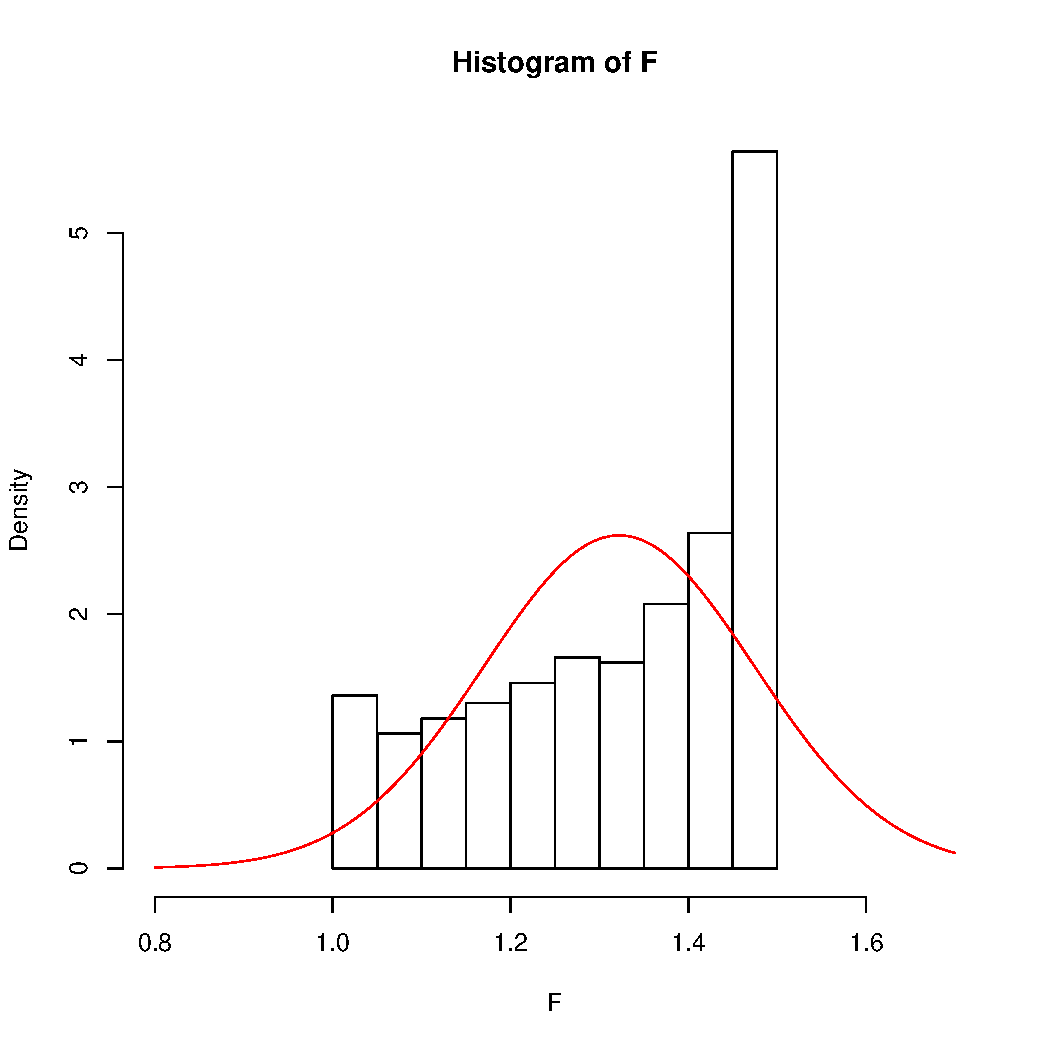
\includegraphics[width=8cm]{Primer_1e+3.pdf}}
\onslide<2>\centerline{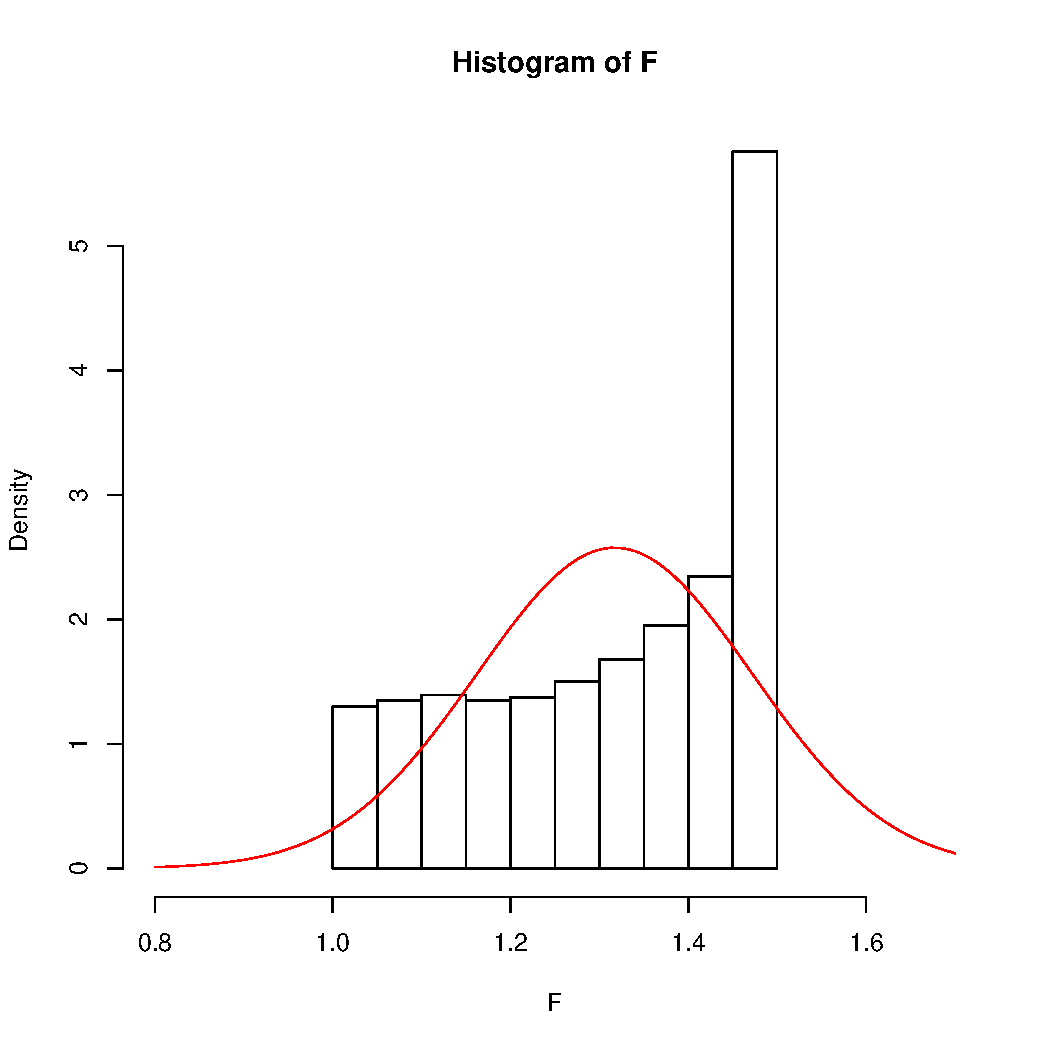
\includegraphics[width=8cm]{Primer_1e+4.pdf}}
\onslide<3>\centerline{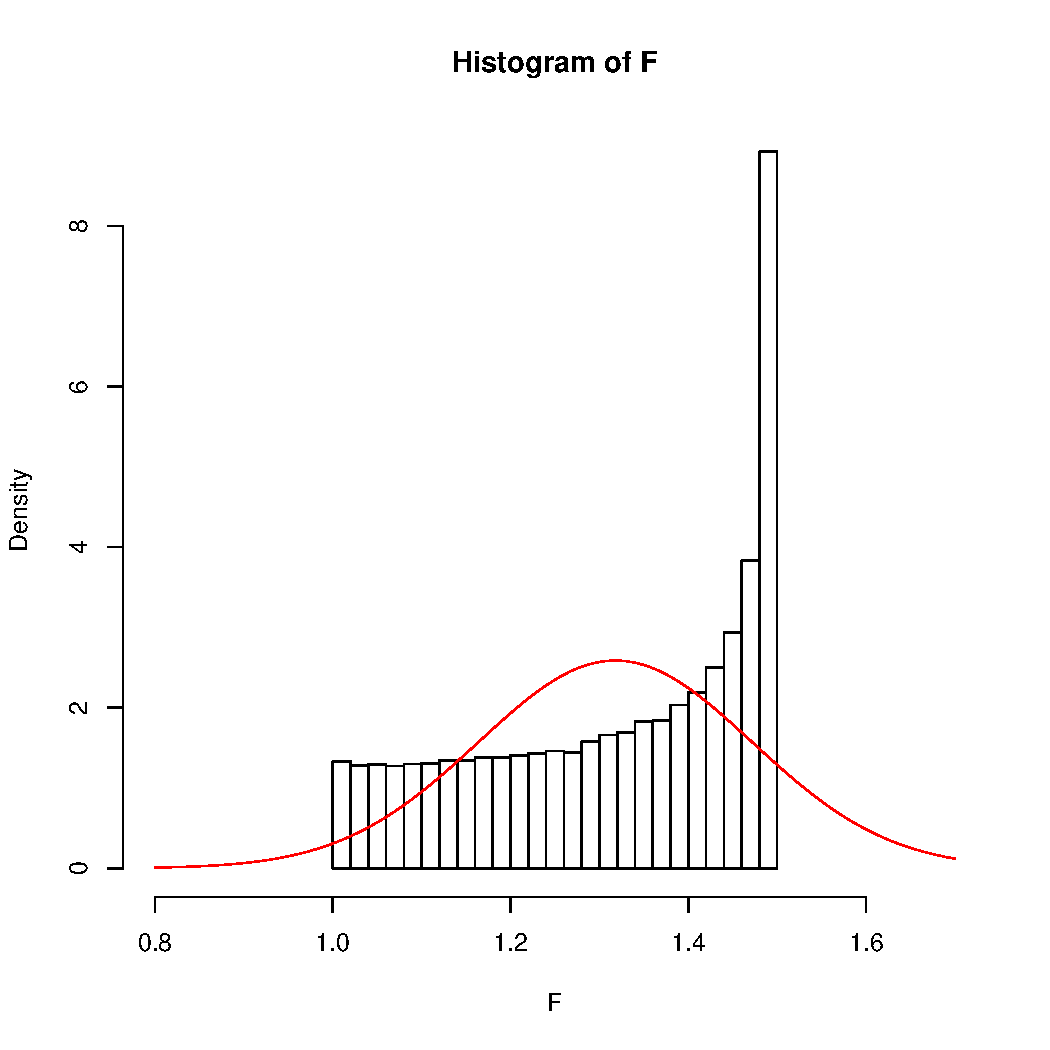
\includegraphics[width=8cm]{Primer_1e+5.pdf}}
\onslide<4>\centerline{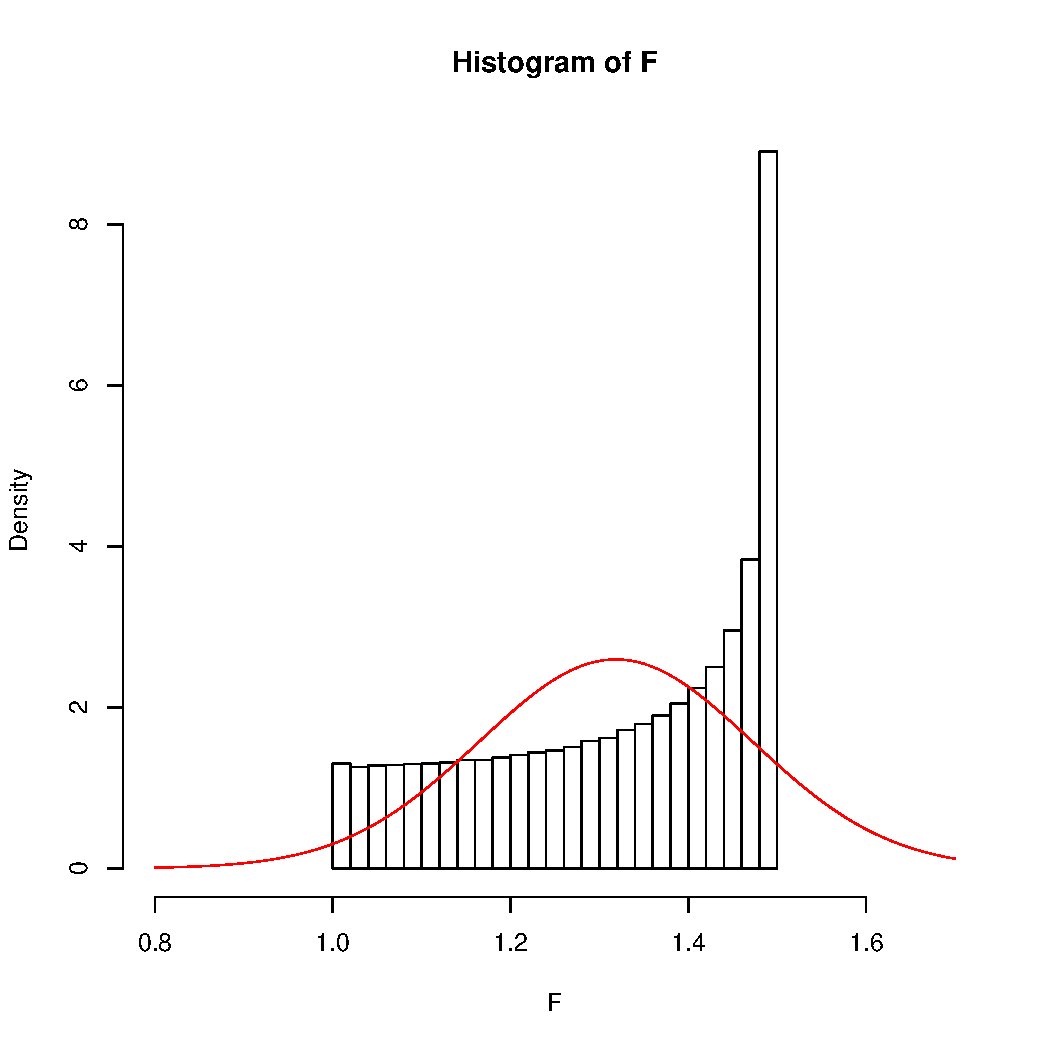
\includegraphics[width=8cm]{Primer_1e+6.pdf}}
\onslide<5>\centerline{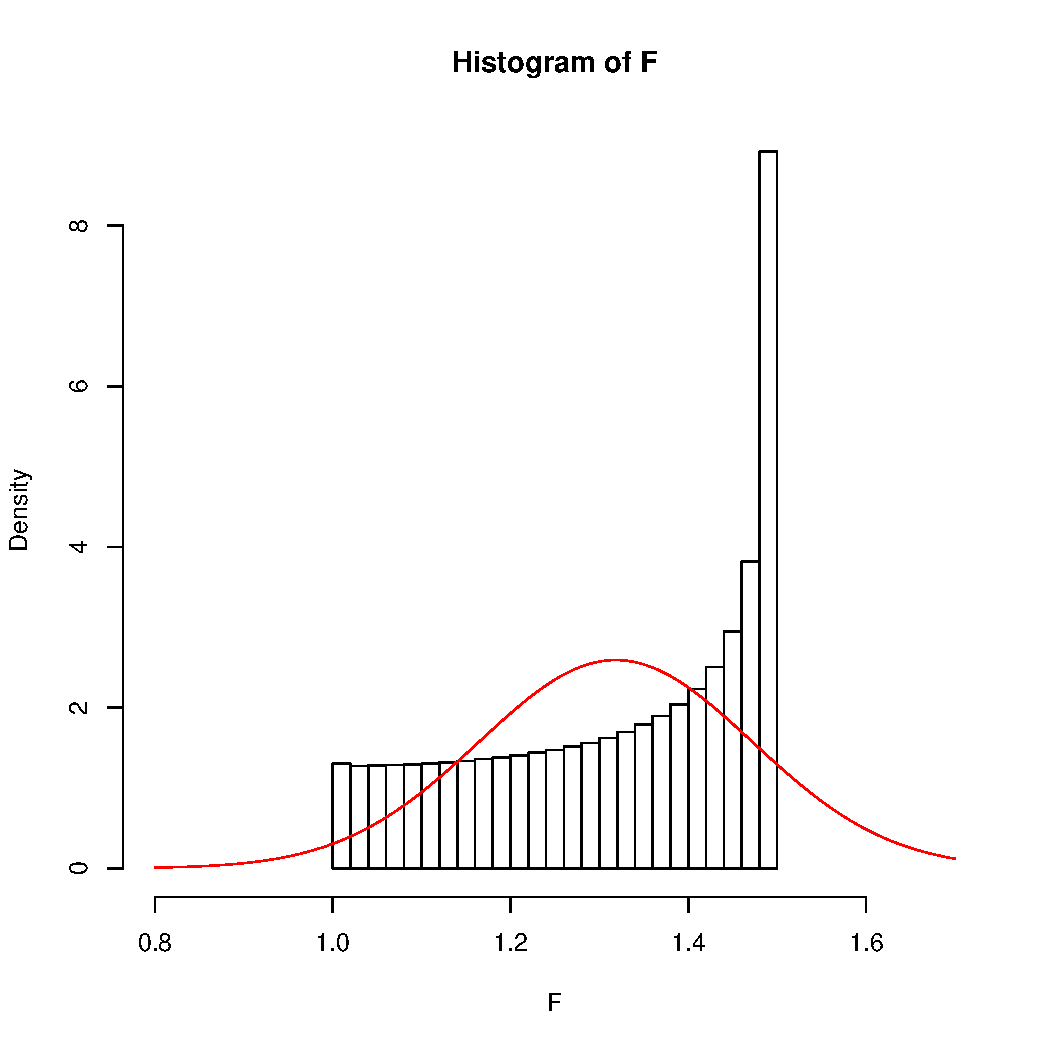
\includegraphics[width=8cm]{Primer_1e+7.pdf}}

\end{overprint}
\end{figure}

\end{frame}

\begin{frame}{Time}
\begin{itemize}
\item $n=2, r=2$: $15,06s$
\item $n=2, r=20$: $19,22s$
\item $n=10,r=20$: $69,25s$
\item $n=\{2,\dots,10\},  r=\{1, \dots,10\}$: $2123,33s -35min$
\item $n=60, r=20$: $21,21min$
\end{itemize}
One table can be generated in $\sim 3h.$
\end{frame}

\begin{frame}{Goals and plans}

\only<1>{\textbf{Main goal:} Generate three tables\\}
\only<1>{\textbf{Work done so far:} Generated all the tables\\}
 \textbf{Plans:} \\
\begin{itemize}
\item Compare the test to well known tests: 
\begin{itemize}
\item Bartlett's test\only<2>{: $$T=\frac{(nr-k)\ln s_{p}^2 - \sum_{i=1}^{r} (n-1)\ln s_{i}^2}{1+\frac{1}{3(r-1)}( \frac{r}{n-1} -\frac{1}{nr-r})},$$ where $s_p^2$ is the pooled variance $s_p^2=\sum_{i=1}^{r}\frac{(n-1)s_{i}^2}{nr-r}.$}

\item Levene's test \only<2>{: $$W=\frac{(nr-r)\sum_{i=1}^{r} n(\bar{Z_{i.}}-\bar{Z{..}})^2}{(r-1)\sum_{i=1}^{r}\sum_{j=1}^{n}(z_{ij}-\bar{Z_{i.}})^2},$$ where $Z_{ij}=|X_{ij}-\bar{X_j}|$ ($\bar{X_j}$ is the mean of group $j$).}

\item Brown–Forsythe test\only<2>{: $$F=\frac{(nr-r)\sum_{i=1}^{r} n(\tilde{z_{.i}}-\tilde{z{..}})^2}{(r-1)\sum_{i=1}^{r}\sum_{j=1}^{n}(z_{ij}-\tilde{z_{.j}})^2},$$where $z_{ij}=|X_{ij}-\tilde{X_j}|$ ($\tilde{X_j}$ is the median of group $j$).}
\end{itemize}
\only<3>{\item Improve the test (if time permits)}
\end{itemize}

\end{frame}


\end{document}

